\documentclass{report}
\usepackage[T1]{fontenc} % Fontes T1
\usepackage[utf8]{inputenc} % Input UTF8
\usepackage[backend=biber, style=ieee]{biblatex} % para usar bibliografia
\usepackage{csquotes}
\usepackage[portuguese]{babel} %Usar língua portuguesa
\usepackage{blindtext} % Gerar texto automaticamente
\usepackage[printonlyused]{acronym}
\usepackage{hyperref} % para autoref
\usepackage{graphicx}
\usepackage{listings}
\usepackage{color}

\definecolor{keywords}{RGB}{255,0,90}
\definecolor{comments}{RGB}{0,0,113}
\definecolor{red}{RGB}{160,0,0}
\definecolor{green}{RGB}{0,150,0}


\bibliography{bibliografia}


\begin{document}
%%
% Definições
%
\def\titulo{Relatório do 2º Trabalho de Aprofundamento}
\def\data{29/05/2021}
\def\autores{Marco Almeida, Rafael Curado}
\def\autorescontactos{(103440) marco.almeida@ua.pt, (103199) rafael.curado@ua.pt}
\def\versao{1.0}
\def\departamento{DETI - Universidade Aveiro}
\def\empresa{Universidade Aveiro}
\def\logotipo{ua.pdf}
%
%%%%%% CAPA %%%%%%
%
\renewcommand{\contentsname}{Índice}
\begin{titlepage}

\begin{center}
%
\vspace*{50mm}
%
{\Huge \titulo}\\ 
%
\vspace{10mm}
%
{\Large \empresa}\\
%
\vspace{10mm}
%
{\LARGE \autores}\\ 
%
\vspace{30mm}
%
\begin{figure}[h]
\center
\includegraphics{\logotipo}
\end{figure}
%
\vspace{30mm}
\end{center}
%
\begin{flushright}
\versao
\end{flushright}
\end{titlepage}

%%  Página de Título %%
\title{%
{\Huge\textbf{\titulo}}\\
{\Large \departamento\\ \empresa}
}
%
\author{%
    \autores \\
    \autorescontactos
}
%
\date{\data}
%
\maketitle

\pagenumbering{roman}

%%%%%% RESUMO %%%%%%
\begin{abstract}
Este trabalho que nos foi proposto é um "jogo" de adivinhar um número secreto.
Mais propriamente, consiste num servidor que gera um número inteiro aleatório (entre 0 e 100) e um número máximo de tentativas (entre 10 e 30) concedidas aos utilizadores para o adivinhar, e num cliente que permite ao utilizador adivinhar esse número. 
\end{abstract}

%%%%%% Agradecimentos %%%%%%
% Segundo glisc deveria aparecer após conclusão...
\renewcommand{\abstractname}{Agradecimentos}
\begin{abstract}
Queremos agradecer ao nosso professor da unidade curricular de Laboratórios de Informática, António Manuel Adrego da Rocha, por nos ter proposto este trabalho e por nos ter dotado de habilidades para a sua execução.
\end{abstract}


\tableofcontents
% \listoftables     % descomentar se necessário
% \listoffigures    % descomentar se necessário


%%%%%%%%%%%%%%%%%%%%%%%%%%%%%%%
\clearpage
\pagenumbering{arabic}

%%%%%%%%%%%%%%%%%%%%%%%%%%%%%%%%
\chapter{Servidor}
\label{chap.servidor}
\section{Características do servidor}
\begin{itemize}
    \item Se o número de argumentos passados ao programa for inválido, ou seja, se for diferente de 2, imprime uma mensagem de erro e não se inicializa.
        \begin{center}
            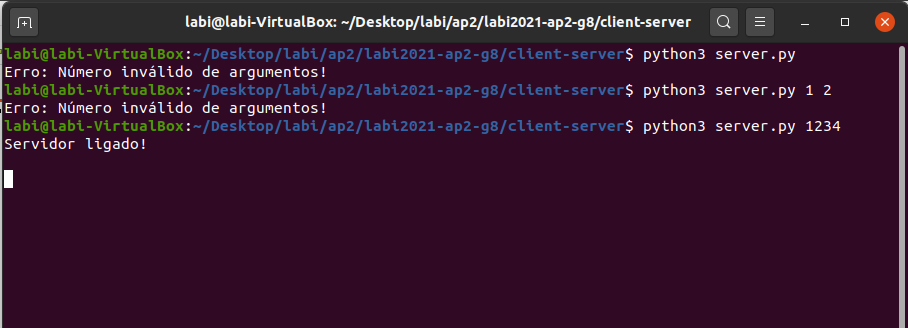
\includegraphics[scale = 0.58]{Imagens/servidor_erro.png}
            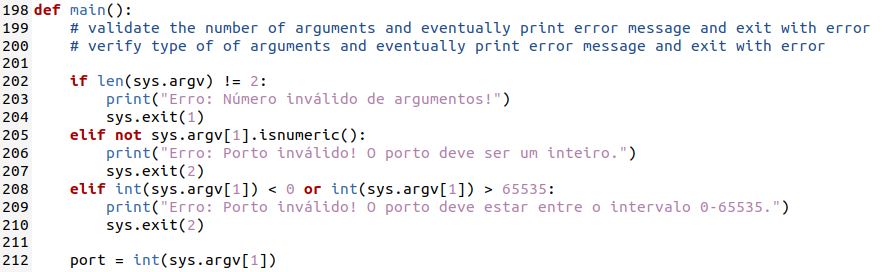
\includegraphics[scale = 0.58]{Imagens/servidor_erro1.png}
        \end{center}
    \item Aceita mais do que um cliente a jogar ao mesmo tempo, desde que não tenha a mesma identificação.
    \item Cria um ficheiro chamado report.csv e vai atualizando-o escrevendo os resultados e pontuações dos clientes quando estes terminam o jogo.
        \begin{center}
            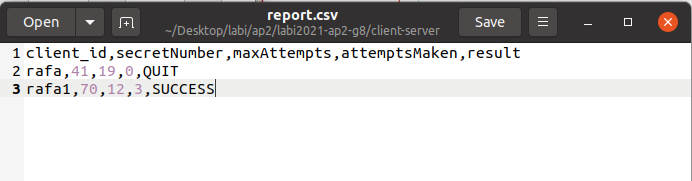
\includegraphics[scale = 0.7]{Imagens/report.png}
        \end{center}
    \item Mesmo que o cliente não tenha adivinhado o número secreto após exceder o número máximo de tentativas, o jogo é considerado sem sucesso.
    \item O servidor imprime mensagens de status sobre os clientes.
        \begin{center}
            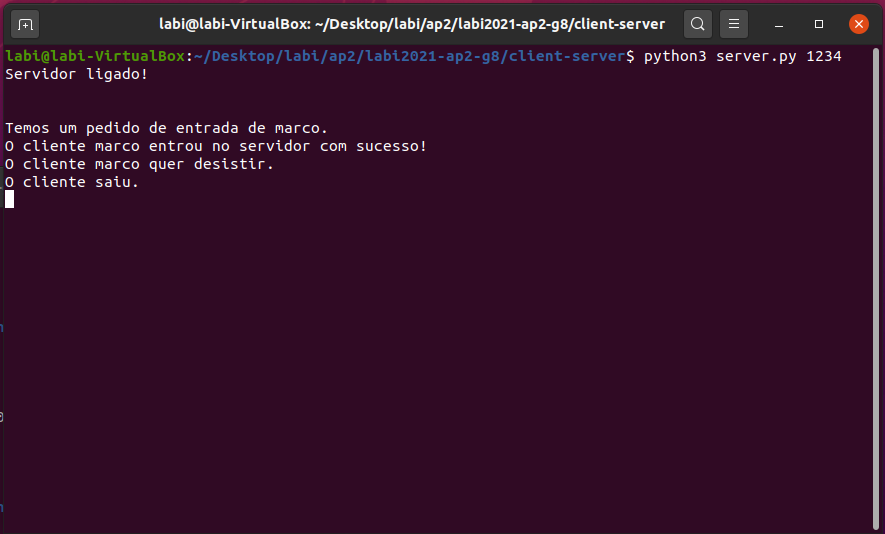
\includegraphics[scale = 0.58]{Imagens/server2.png}
        \end{center}
\end{itemize}

\chapter{Cliente}
\label{chap.cliente}
\section{Características do cliente}
\begin{itemize}
    \item Se o número de argumentos passados ao programa for inválido, ou seja, se for diferente de 3 e se o 3º argumento, que é o porto, for diferente do porto do servidor, imprime uma mensagem de erro e não se inicializa.
        \begin{center}
            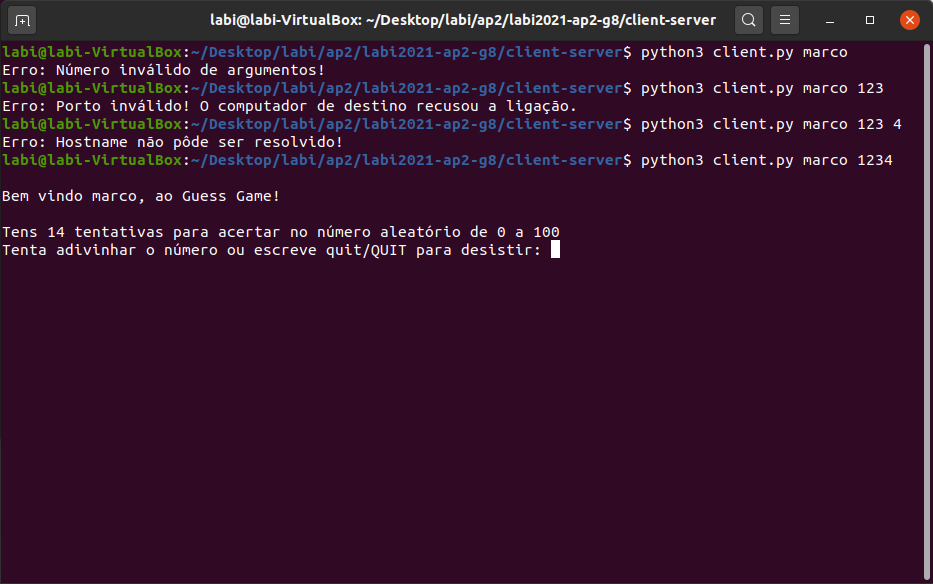
\includegraphics[scale = 0.55]{Imagens/cliente4.png}
            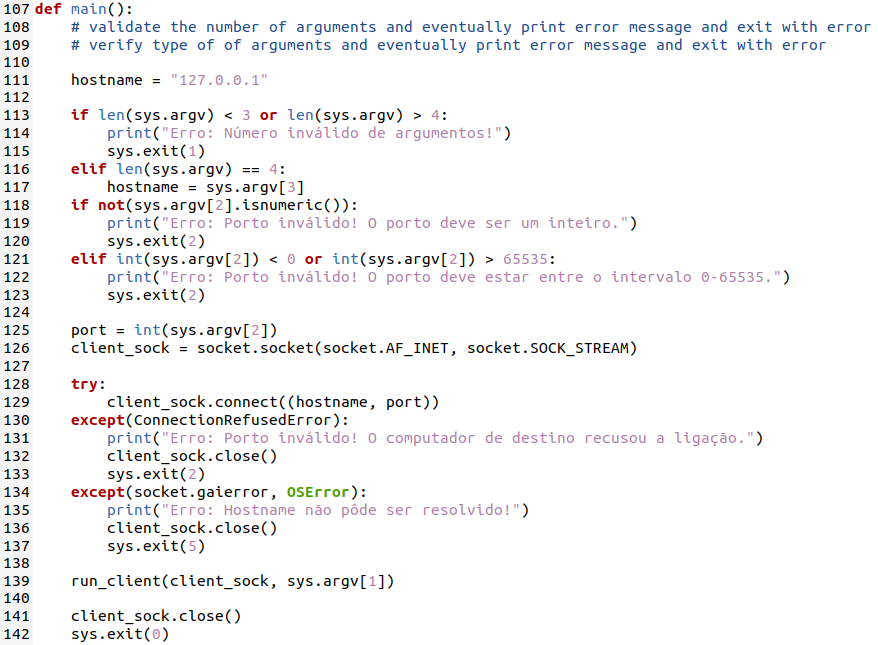
\includegraphics[scale = 0.59]{Imagens/cliente5.png}
        \end{center}
    
    
    \item Pode desistir a qualquer altura do jogo escrevendo "quit" ou "QUIT".
    \item Quando o utilizador adivinha o número secreto o cliente imprime uma mensagem a dizer que acertou, o número de jogadas efetuadas e quantas restavam.
        \begin{center}
            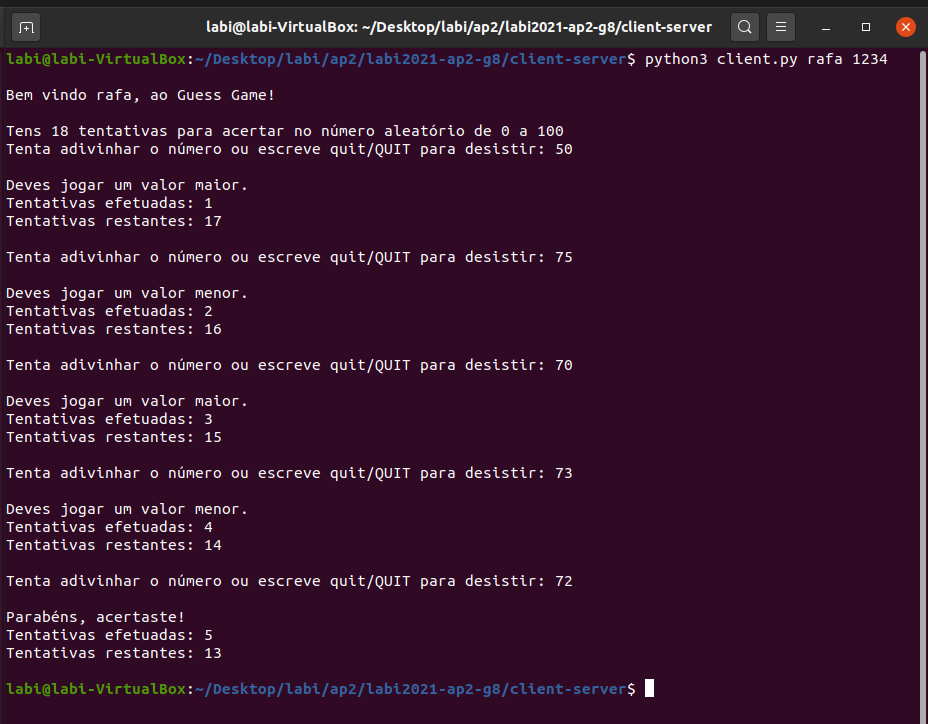
\includegraphics[scale = 0.57]{Imagens/cliente.png}
        \end{center}
    \item Mesmo que o utilizador esgote o número de tentativas sem adivinhar o número secreto o jogo continua até o utilizador acertar.
        \begin{center}
            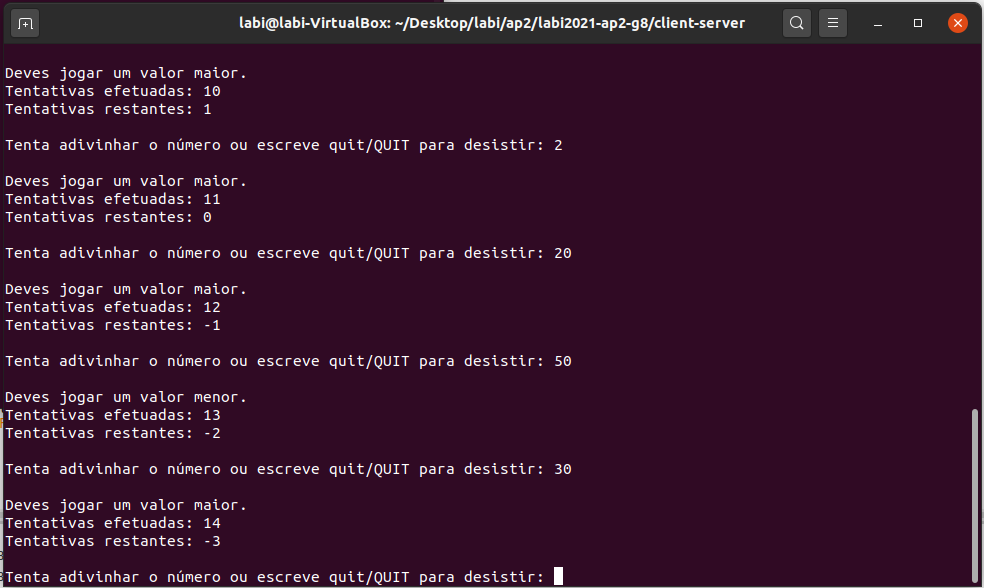
\includegraphics[scale = 0.54]{Imagens/cliente1.png}
        \end{center}
    \item O cliente não aceita entradas que não sejam números inteiros entre 0 e 100, exceto o "quit". Caso isso aconteça, o número de tentativas efetuadas e o número de tentativas restantes não varia.
        \begin{center}
            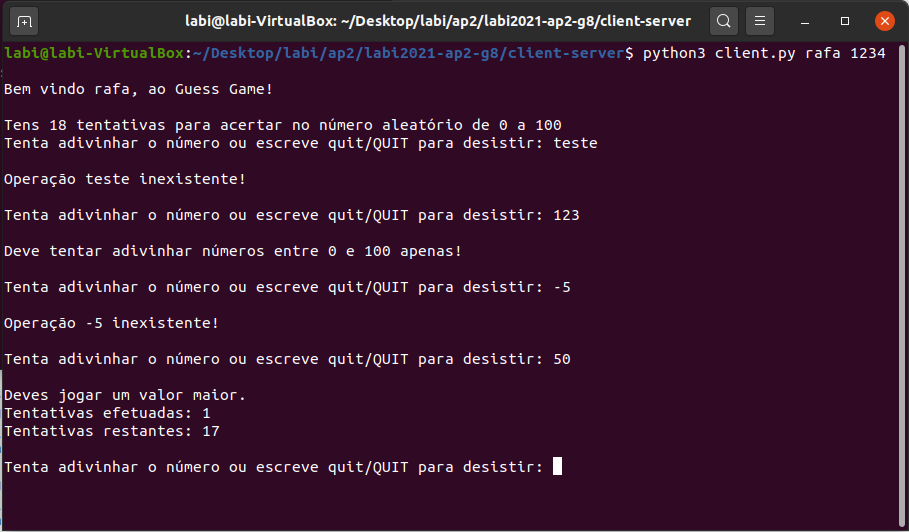
\includegraphics[scale = 0.58]{Imagens/cliente2.png}
            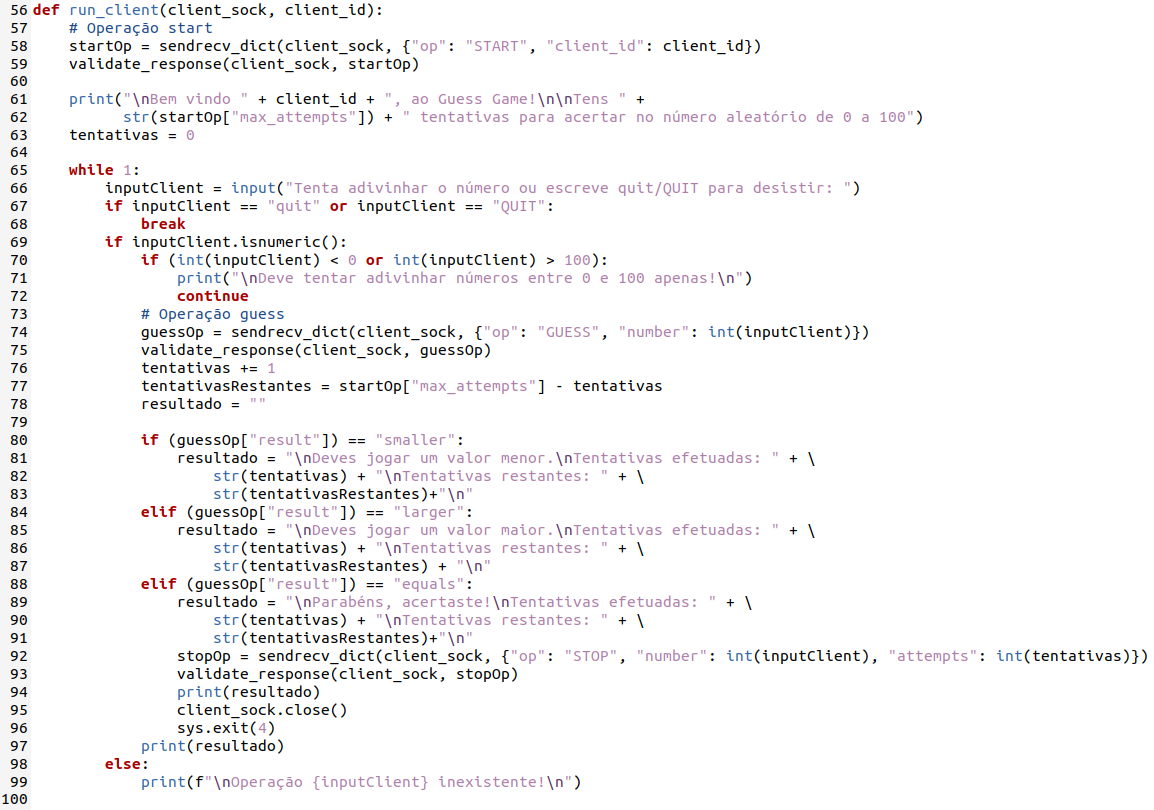
\includegraphics[scale = 0.5]{Imagens/cliente3.png}
        \end{center}
\end{itemize}


\chapter{Testes}
\label{chap.testes}
Aqui podemos analisar um teste feito corretamente, ou seja, com o número correto de argumentos passados ao programa do servidor ("server.py") e ao programa do cliente ("client.py").

\begin{center}
    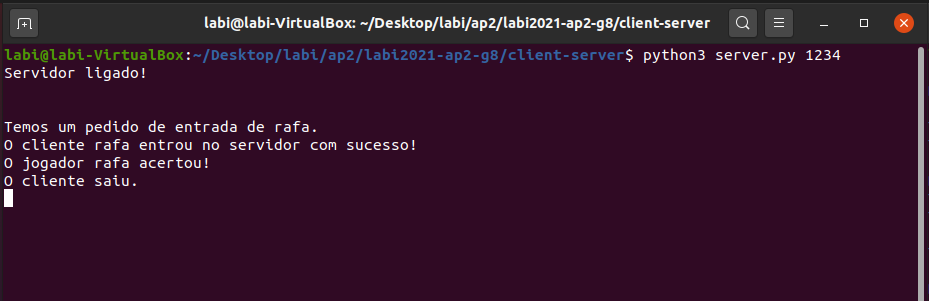
\includegraphics[scale = 0.52]{Imagens/servidor.png}
    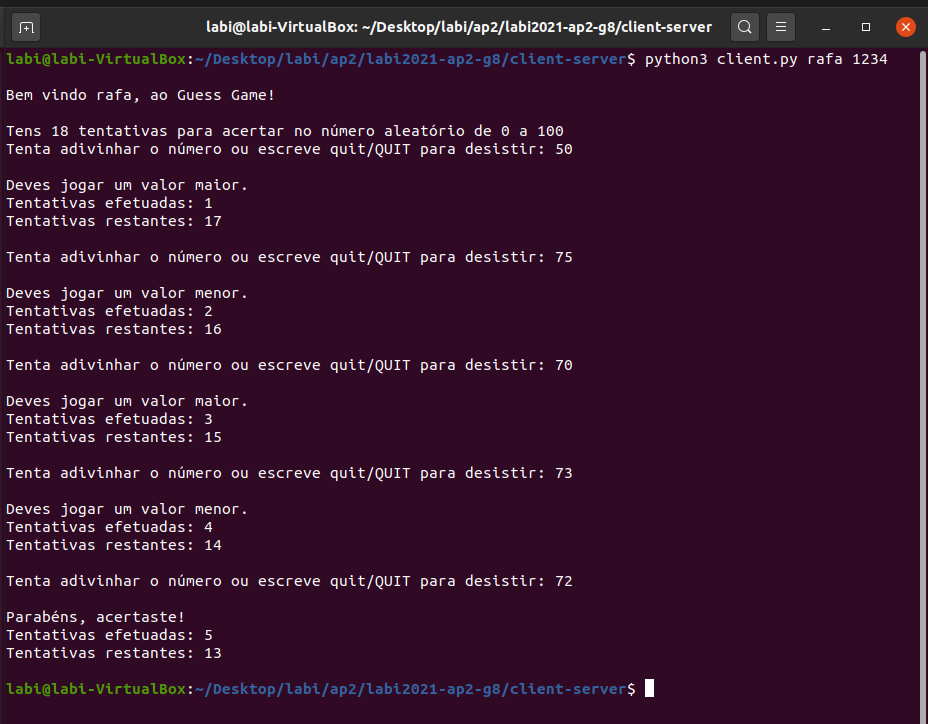
\includegraphics[scale = 0.52]{Imagens/cliente.png}
\end{center}

\chapter*{Contribuições dos autores}
A dedicação e conhecimentos adquiridos nas aulas por parte de ambos os alunos foram essenciais para a realização deste trabalho, pelo que o aluno MA se destacou na execução do mesmo. Posto isto, o aluno MA contribuiu cerca de 60 \% e o aluno RC contribuiu cerca de 40 \% .



%%%%%%%%%%%%%%%%%%%%%%%%%%%%%%%%%

\begin{acronym}
\acro{ua}[UA]{Universidade de Aveiro}
\acro{miect}[MIECT]{Mestrado Integrado em Engenharia de Computadores e Telemática}
\acro{lei}[LEI]{Licenciatura em Engenharia Informática}
\acro{glisc}[GLISC]{Grey Literature International Steering Committee}
\end{acronym}


%%%%%%%%%%%%%%%%%%%%%%%%%%%%%%%%%
\printbibliography

\end{document}
